\documentclass[aspectratio=169]{../latex_main/tntbeamer}  % you can pass all options of the beamer class, e.g., 'handout' or 'aspectratio=43'
\usepackage{dsfont}
\usepackage{bm}
\usepackage[english]{babel}
\usepackage[T1]{fontenc}
%\usepackage[utf8]{inputenc}
\usepackage{graphicx}
\graphicspath{ {./figures/} }
\usepackage{algorithm}
\usepackage[ruled,vlined,algo2e,linesnumbered]{algorithm2e}
\usepackage{hyperref}
\usepackage{booktabs}
\usepackage{mathtools}

\usepackage{amsmath,amssymb}

\DeclareMathOperator*{\argmax}{arg\,max}
\DeclareMathOperator*{\argmin}{arg\,min}

\usepackage{amsbsy}
\newcommand{\vect}[1]{\bm{#1}}
%\newcommand{\vect}[1]{\boldsymbol{#1}}

\usepackage{pgfplots}
\pgfplotsset{compat=1.16}
\usepackage{tikz}
\usetikzlibrary{trees} 
\usetikzlibrary{shapes.geometric}
\usetikzlibrary{positioning,shapes,shadows,arrows,calc,mindmap}
\usetikzlibrary{positioning,fadings,through}
\usetikzlibrary{decorations.pathreplacing}
\usetikzlibrary{intersections}
\pgfdeclarelayer{background}
\pgfdeclarelayer{foreground}
\pgfsetlayers{background,main,foreground}
\tikzstyle{activity}=[rectangle, draw=black, rounded corners, text centered, text width=8em]
\tikzstyle{data}=[rectangle, draw=black, text centered, text width=8em]
\tikzstyle{myarrow}=[->, thick, draw=black]

% Define the layers to draw the diagram
\pgfdeclarelayer{background}
\pgfdeclarelayer{foreground}
\pgfsetlayers{background,main,foreground}

% Requires XeLaTeX or LuaLaTeX
%\usepackage{unicode-math}

\usepackage{fontspec}
%\setsansfont{Arial}
\setsansfont{RotisSansSerifStd}[ 
Path=../latex_main/fonts/,
Extension = .otf,
UprightFont = *-Regular,  % or *-Light
BoldFont = *-ExtraBold,  % or *-Bold
ItalicFont = *-Italic
]
\setmonofont{Cascadia Mono}[
Scale=0.8
]

% scale factor adapted; mathrm font added (Benjamin Spitschan @TNT, 2021-06-01)
%\setmathfont[Scale=1.05]{Libertinus Math}
%\setmathrm[Scale=1.05]{Libertinus Math}

% other available math fonts are (not exhaustive)
% Latin Modern Math
% XITS Math
% Libertinus Math
% Asana Math
% Fira Math
% TeX Gyre Pagella Math
% TeX Gyre Bonum Math
% TeX Gyre Schola Math
% TeX Gyre Termes Math

% Literature References
\newcommand{\lit}[2]{\href{#2}{\footnotesize\color{black!60}[#1]}}

%%% Beamer Customization
%----------------------------------------------------------------------
% (Don't) Show sections in frame header. Options: 'sections', 'sections light', empty
\setbeamertemplate{headline}{empty}

% Add header logo for normal frames
\setheaderimage{
	% 
\includegraphics[height=\logoheight]{figures/TNT_darkv4.pdf}
	
\includegraphics[height=\logoheight]{../latex_main/figures/luh_logo_rgb_0_80_155.pdf}
	% 
\includegraphics[height=\logoheight]{figures/logo_tntluh.pdf}
}

% Header logo for title page
\settitleheaderimage{
	% 
\includegraphics[height=\logoheight]{figures/TNT_darkv4.pdf}
	
\includegraphics[height=\logoheight]{../latex_main/figures/luh_logo_rgb_0_80_155.pdf}
	% 
\includegraphics[height=\logoheight]{figures/logo_tntluh.pdf}
}

% Title page: tntdefault 
\setbeamertemplate{title page}[tntdefault]  % or luhstyle
% Add optional title image here
%\addtitlepageimagedefault{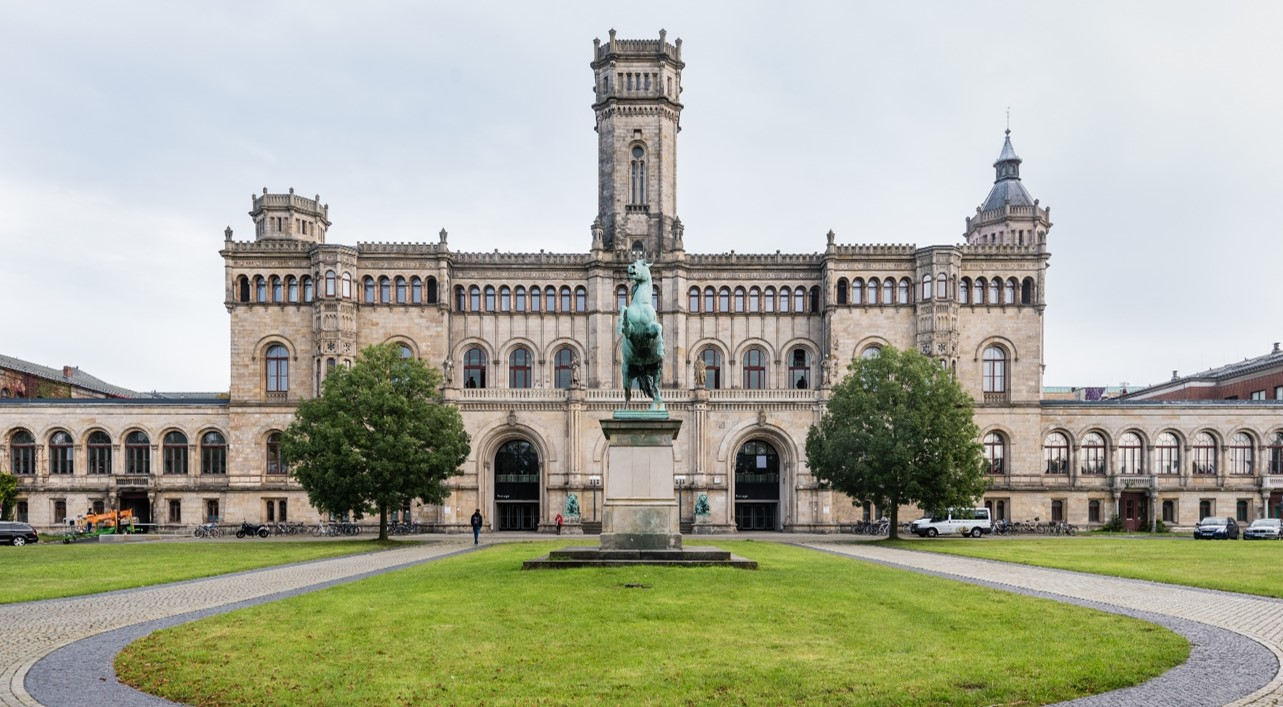
\includegraphics[width=0.65\textwidth]{figures/luh_default_presentation_title_image.jpg}}

% Title page: luhstyle
% \setbeamertemplate{title page}[luhstyle]
% % Add optional title image here
% \addtitlepageimage{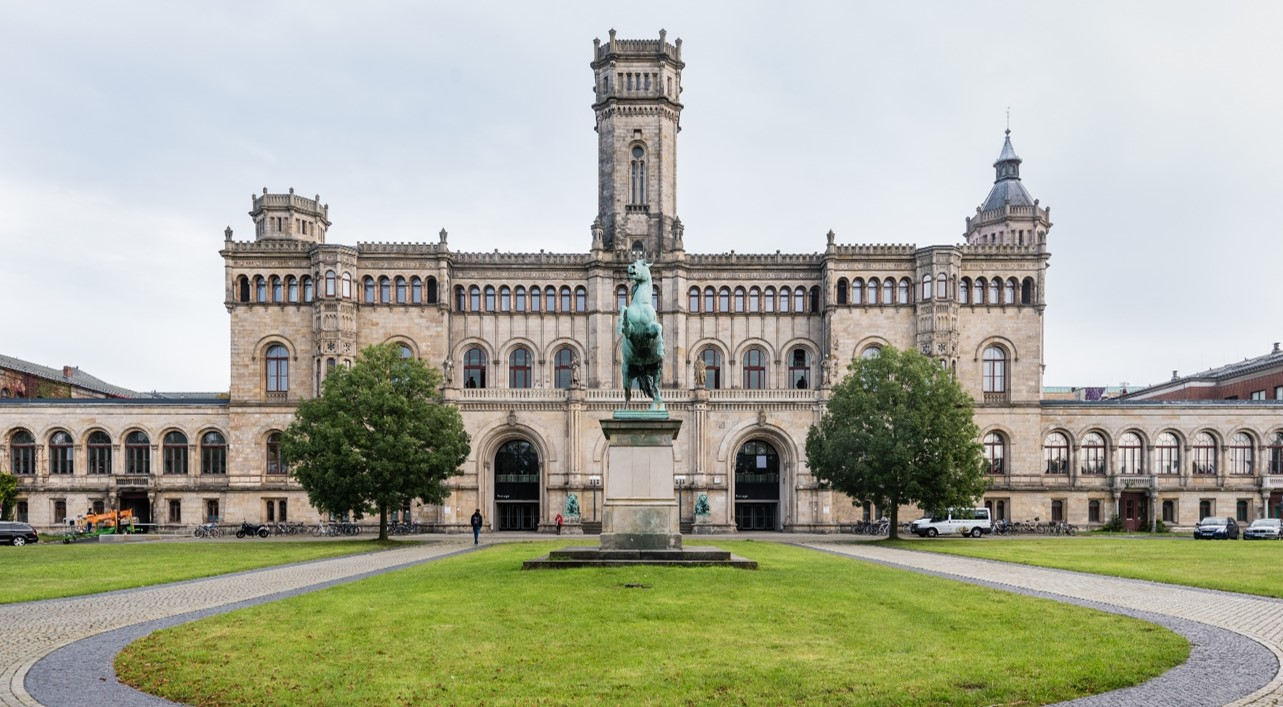
\includegraphics[width=0.75\textwidth]{figures/luh_default_presentation_title_image.jpg}}

\author[Abedjan \& Lindauer]{Ziawasch Abedjan \& Marius Lindauer\\[1em]
	
\includegraphics[height=\logoheight]{../latex_main/figures/luh_logo_rgb_0_80_155.pdf}\qquad
	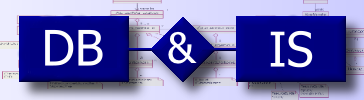
\includegraphics[height=\logoheight]{../latex_main/figures/DBIS_Kurzlogo.png}\qquad

\includegraphics[height=\logoheight]{../latex_main/figures/TNT_darkv4}\qquad

\includegraphics[height=\logoheight]{../latex_main/figures/L3S.jpg}	}
\date{Summer Term 2022; \hspace{0.5em} {
\includegraphics[height=1.5em]{../latex_main/figures/Cc-by-nc-sa_icon.svg.png}}; based on \href{https://ds100.org/fa21/}{[DS100]}
}


%%% Custom Packages
%----------------------------------------------------------------------
% Create dummy content
\usepackage{blindtext}

% Adds a frame with the current page layout. Just call \layout inside of a frame.
\usepackage{layout}


%%% Macros
%\renewcommand{\vec}[1]{\mathbf{#1}}
% \usepackage{bm}
%\let\vecb\bm

\title[Introduction]{DS: Logistic Regression, Classification}
\subtitle{Visual metrics}

\graphicspath{ {./figure/} }
%\institute{}


\begin{document}
	
	\maketitle
	\begin{frame}{The effect of thresholds}
	    \begin{itemize}
	        \item Our choice of threshold impacts our model’s:
	        \begin{itemize}
	            \item Accuracy.
	            \item Precision.
	            \item Recall.
	        \end{itemize}
	        \item Let’s explore!
	    \end{itemize}
	\end{frame}
	
	
	\begin{frame}{Accuracy vs. threshold}
	    \begin{columns}
	        \begin{column}{.5\textwidth}
	             \begin{itemize}
	                 \item If our threshold is too high, we will have many false negatives.
	                 \item If our threshold is too low, we will have many false positives.
	                 \item Thus, we’d expect our accuracy to be maximized when our threshold is near 0.5 in a typical setting.
	                 \begin{itemize}
	                     \item Not always the case.
	                 \end{itemize}
	             \end{itemize}   
	        \end{column}
	        
	        
	        \begin{column}{.5\textwidth}
	                \begin{figure}
	                    \centering
	                    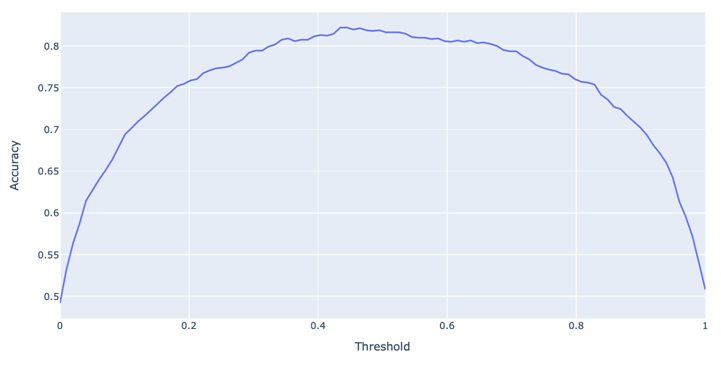
\includegraphics[scale=.6]{Bild17}
	                \end{figure}
	                Accuracy vs. threshold for our two feature NBA model, $ P(Y=1|x) = \sigma (\theta_0  + \theta_1 \cdot FG\_PCT\_DIFF + \theta_2 \cdot PF\_DIFF)$
	        \end{column}
	        
	    \end{columns}
	\end{frame}
	
	
	
	\begin{frame}{Precision vs. threshold}
	    \begin{columns}
	        \begin{column}{.5\textwidth}
	             \begin{itemize}
	                 \item As we increase our threshold, we have fewer and fewer false positives.
	                 \item Thus, precision tends to increase.
	             \end{itemize} 
	             
	             \begin{align*}
	                 \text{Precision} &= \frac{\text{True Positives}}{\text{True Positives} + \text{False Positives}}\\
	                 &= \frac{\text{True Positives}}{\text{Predicted True}}
	             \end{align*}
	                 \hspace{1cm} 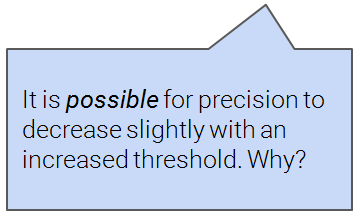
\includegraphics[scale=.25]{Bild19}
	        \end{column}
	        
	        
	        \begin{column}{.5\textwidth}
	                \begin{figure}
	                    \centering
	                    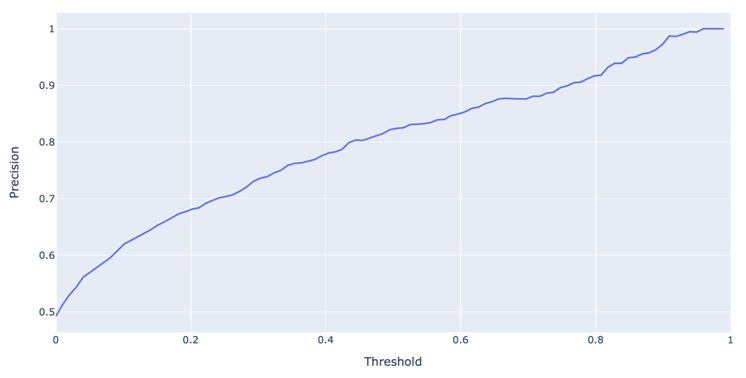
\includegraphics[scale=.6]{Bild18}
	                \end{figure}
	                
	                
	        \end{column}
	        
	    \end{columns}
	\end{frame}
	
	
	\begin{frame}{Recall vs. threshold}
	    \begin{columns}
	        \begin{column}{.5\textwidth}
	             \begin{itemize}
	                 \item As we increase our threshold, we have more and more false negatives.
	                 \item Thus, recall tends to decrease.
	             \end{itemize} 
	             
	             \begin{align*}
	                 \text{Recall} &= \frac{\text{True Positives}}{\text{True Positives} + \text{False Negatives}}\\
	                 &= \frac{\text{True Positives}}{\text{Actually True}}
	             \end{align*}
	                 \hspace{3cm} 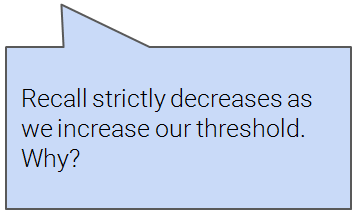
\includegraphics[scale=.23]{Bild20}
	        \end{column}
	        
	        
	        \begin{column}{.5\textwidth}
	                \begin{figure}
	                    \centering
	                    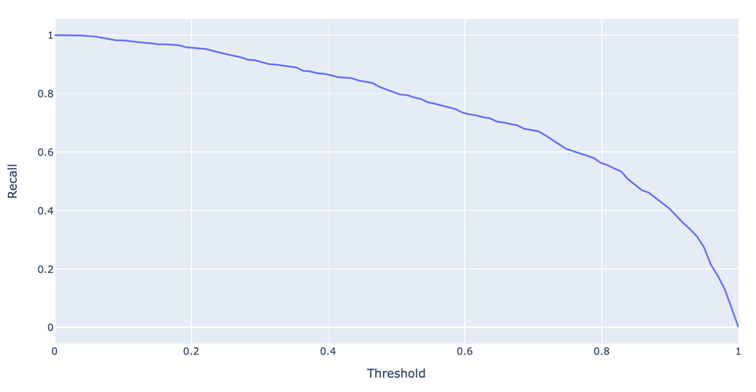
\includegraphics[scale=.6]{Bild21}
	                \end{figure}
	                
	                
	        \end{column}
	        
	    \end{columns}
	\end{frame}
	
	
	\begin{frame}{.}
	    \begin{figure}
	        \centering
	        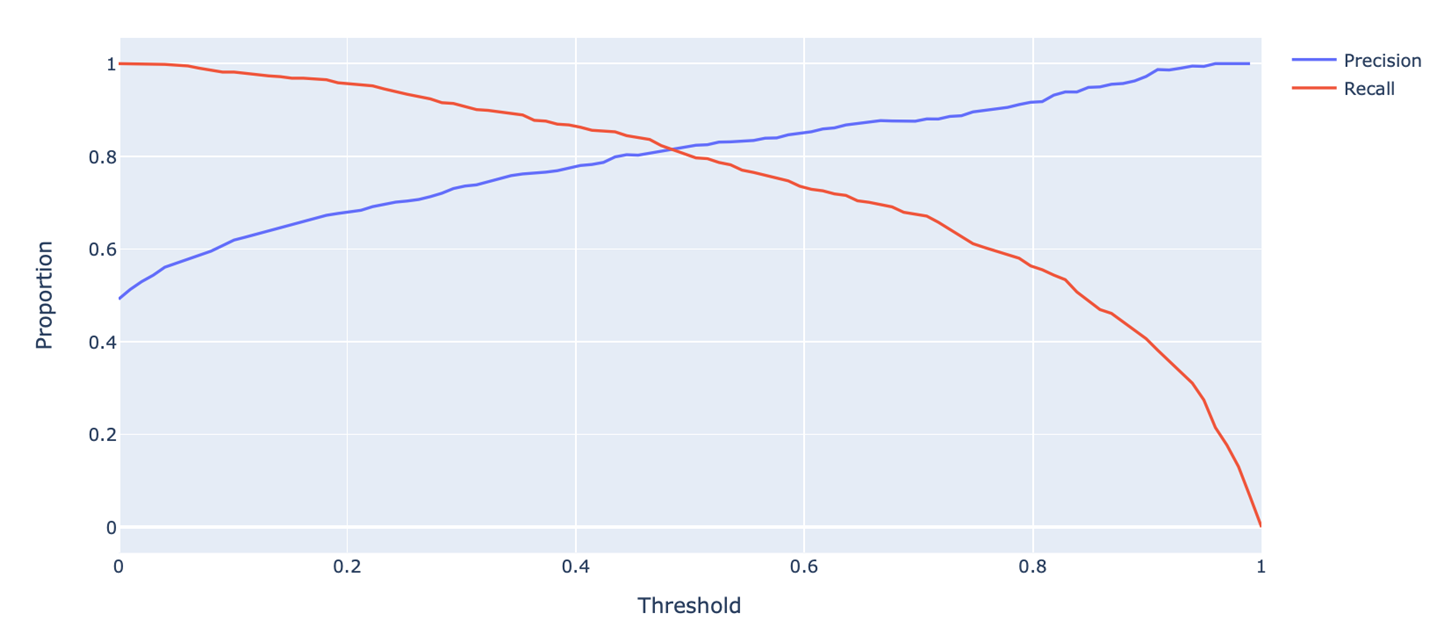
\includegraphics[scale=.6]{Bild22}
	    \end{figure}
	\end{frame}
	
	
	
	\begin{frame}{Precision-recall curves}
	    \begin{columns}
	        \begin{column}{.5\textwidth}
	        We can also plot precision vs. recall, for all possible thresholds.\\
	        \bigskip
	        Question: 
	             \begin{itemize}
	                 \item Which part of this curve corresponds to T = 0.9?
	                 \item Which part of this curve corresponds to T = 0.1?
	             \end{itemize} 
	        \end{column}
	        
	        
	        \begin{column}{.5\textwidth}
	                \begin{figure}
	                    \centering
	                    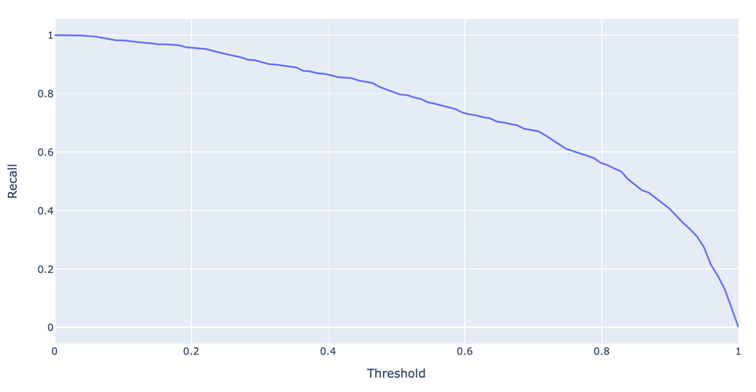
\includegraphics[scale=.6]{Bild21}
	                \end{figure}
	                
	                
	        \end{column}
	        
	    \end{columns}
	\end{frame}
	
	
	\begin{frame}{Precision-recall curves}
	    \begin{columns}
	        \begin{column}{.5\textwidth}
	        We can also plot precision vs. recall, for all possible thresholds.\\
	        \bigskip
	        Answer: 
	             \begin{itemize}
	                 \item Threshold decreases from the top left to the bottom right.
	                 \item In the notebook, there’s an interactive version of this plot.
	             \end{itemize} 
	        \end{column}
	        
	        
	        \begin{column}{.5\textwidth}
	                \begin{figure}
	                    \centering
	                    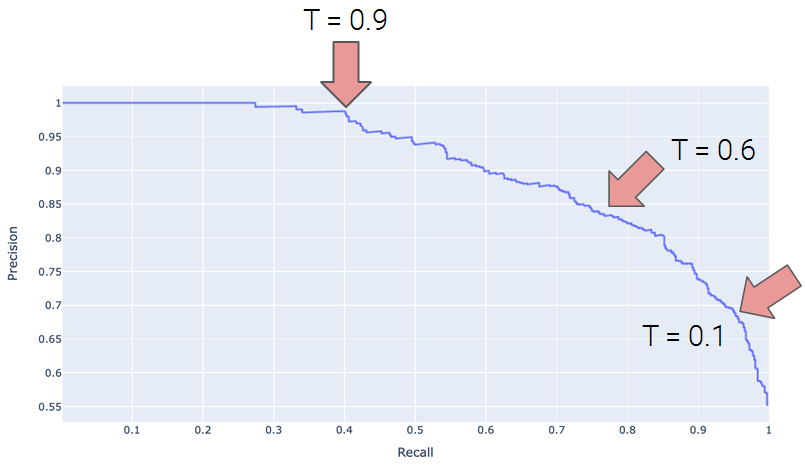
\includegraphics[scale=.35]{Bild24}
	                \end{figure}
	                
	                
	        \end{column}
	        
	    \end{columns}
	\end{frame}
	
	
	\begin{frame}{Precision-recall curves}
	    \begin{columns}
	        \begin{column}{.5\textwidth}
	        The “perfect classifier” is one with precision of 1 and recall of 1.
	             \begin{itemize}
	                 \item We want our PR curve to be as close to the “top right” of this graph as possible.
	                 \item One way to compare our model is to compute its area under curve (AUC).
	                 \begin{itemize}
	                     \item The area under the “optimal PR curve” is 1.
	                     \item More commonly, we look at the area under ROC curve.
	                 \end{itemize}
	             \end{itemize} 
	        \end{column}
	        
	        
	        \begin{column}{.5\textwidth}
	                \begin{figure}
	                    \centering
	                    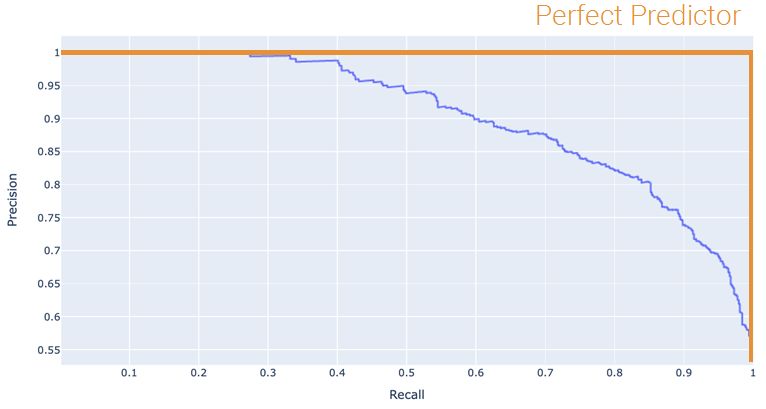
\includegraphics[scale=.35]{Bild25}
	                \end{figure}
	                
	                
	        \end{column}
	        
	    \end{columns}
	\end{frame}
	
	
	\begin{frame}{Other metrics}
	    \begin{columns}
	        \begin{column}{.5\textwidth}
    	        False Positive Rate (FPR):
	             \begin{itemize}
	                 \item FP / (FP + TN)
	                 \item “What proportion of innocent people did I convict?”
	             \end{itemize}
	             True Positive Rate (TPR):
	             \begin{itemize}
	                 \item TP / (TP + FN)
	                 \item “What proportion of guilty people did I convict?”
	                 \item Same thing as recall.
	             \end{itemize}
	        \end{column}
	        
	        
	        \begin{column}{.5\textwidth}
	                \begin{figure}
	                    \centering
	                    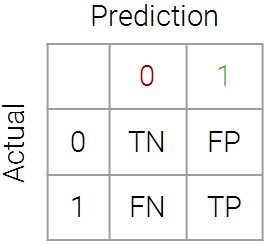
\includegraphics[scale=.55]{Bild12}\\
	                    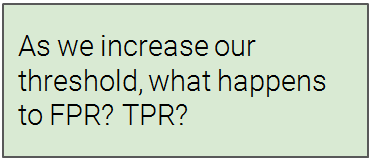
\includegraphics[scale=.5]{Bild26}
	                \end{figure}
	                
	                
	        \end{column}
	        
	    \end{columns}
	\end{frame}
	
	
	\begin{frame}{ROC curves}
	    \begin{columns}
	        \begin{column}{.5\textwidth}
    	        A ROC curve plots TPR vs. FPR.
	             \begin{itemize}
	                 \item As we increase our threshold, both TPR and FPR decrease.
	                 \begin{itemize}
	                     \item A decreased TPR is bad (detecting fewer positives).
	                     \item A decreased FPR is good (fewer false positives).
	                     \item Tradeoff!
	                 \end{itemize}
	             \end{itemize}
	             \begin{itemize}
	                 \item ROC stands for “Receiver Operating Characteristic.”
	             \end{itemize}
	        \end{column}
	        
	        
	        \begin{column}{.5\textwidth}
	                \begin{figure}
	                    \centering
	                    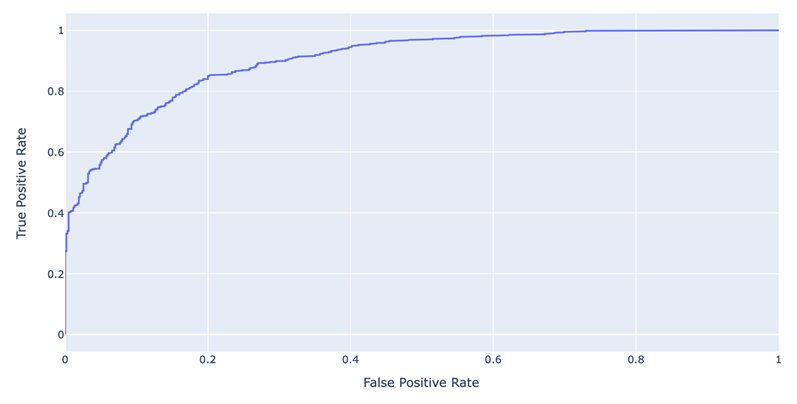
\includegraphics[scale=.55]{Bild27}
	                \end{figure}
	                
	                
	        \end{column}
	        
	    \end{columns}
	\end{frame}
	
	
	\begin{frame}{ROC curves}
	    \begin{columns}
	        \begin{column}{.5\textwidth}
    	        A ROC curve plots TPR vs. FPR.
	             \begin{itemize}
	                 \item As we increase our threshold, both TPR and FPR decrease.
	                 \begin{itemize}
	                     \item A decreased TPR is bad (detecting fewer positives).
	                     \item A decreased FPR is good (fewer false positives).
	                     \item Tradeoff!
	                 \end{itemize}
	             \end{itemize}
	             \begin{itemize}
	                 \item ROC stands for “Receiver Operating Characteristic.”
	             \end{itemize}
	        \end{column}
	        
	        
	        \begin{column}{.5\textwidth}
	                \begin{figure}
	                    \centering
	                    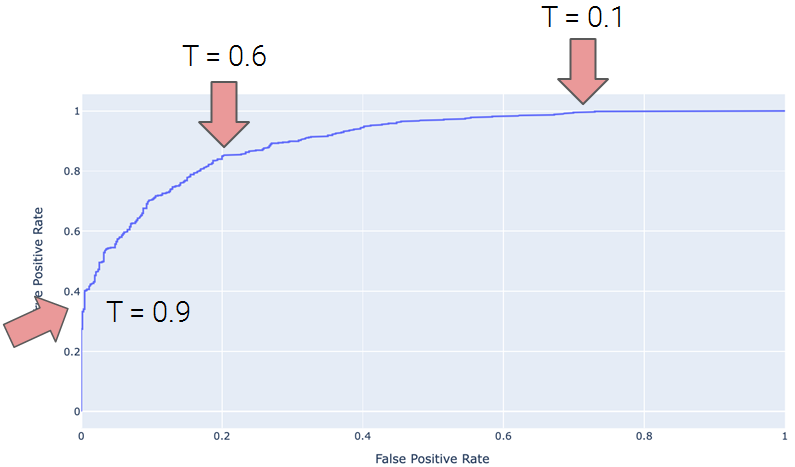
\includegraphics[scale=.35]{Bild28}
	                \end{figure}
	                
	                
	        \end{column}
	        
	    \end{columns}
	\end{frame}
	
	
	
	\begin{frame}{ROC curves and AUC}
	    \begin{columns}
	        \begin{column}{.5\textwidth}
    	      The “perfect” classifier is the one that has a TPR of 1, and FPR of 0.
	             \begin{itemize}
	                 \item We want our logistic regression model to match that as well as possible.
	                 \item We want our ROC curve to be as close to the “top left” of this graph as possible.
	                 \item We can compute the area under curve (AUC) of our model.
	             
	             \begin{itemize}
	                 \item Best possible AUC = 1.
	                 \item Terrible AUC = 0.5 (randomly guessing).
	             \end{itemize}
	             \end{itemize}
	        \end{column}
	        
	        
	        \begin{column}{.5\textwidth}
	                \begin{figure}
	                    \centering
	                    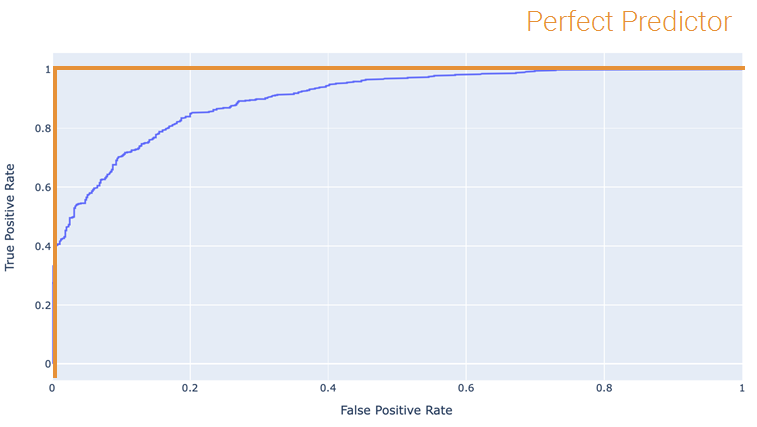
\includegraphics[scale=.35]{Bild29}
	                \end{figure}
	                
	                
	        \end{column}
	        
	    \end{columns}
	\end{frame}
	
	
	\begin{frame}{ROC curves and AUC}
	    \begin{columns}
	        \begin{column}{.5\textwidth}
	             \begin{itemize}
	                 \item We can compute the area under curve (AUC) of our model.
	                 \begin{itemize}
	                     \item Different AUCs for both ROC curves and PR curves, but ROC is more common.
	                 \end{itemize}
	                 \item Best possible AUC = 1.
	                 \item Terrible AUC = 0.5.
	                 \begin{itemize}
	                    \item Random predictors have an AUC of around 0.5. Why?
	                 \end{itemize}
	                 \item Your model’s AUC: somewhere between 0.5 and 1.
	             \end{itemize}
	        \end{column}
	        
	        
	        \begin{column}{.5\textwidth}
	                \begin{figure}
	                    \centering
	                    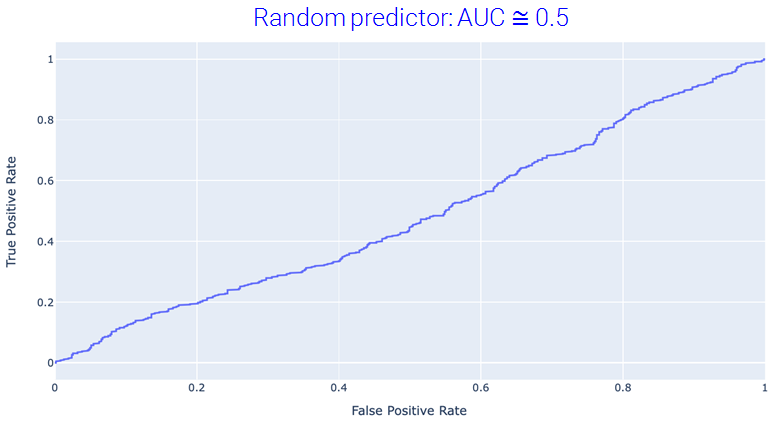
\includegraphics[scale=.35]{Bild30}
	                \end{figure}
	                
	                
	        \end{column}
	        
	    \end{columns}
	\end{frame}
	
	
	\begin{frame}{Common techniques for evaluating classifiers}
	    \begin{columns}
	        \begin{column}{.5\textwidth}
	            Numerical assessments:
	             \begin{itemize}
	                 \item Accuracy, precision, recall, TPR, FPR.
	                 \item Area under curve (AUC), for both PR and ROC.
	             \end{itemize}
	             Visualizations:
	             \begin{itemize}
	                 \item Confusion matrices.
	                 \item Precision/recall curves.
	                 \item ROC curves.
	             \end{itemize}
	             \begin{figure}
	                    \centering
	                    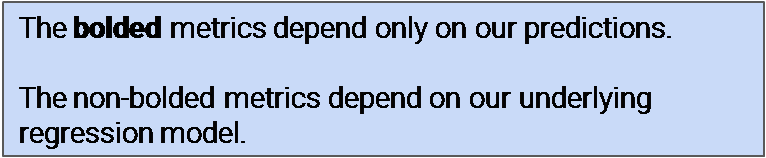
\includegraphics[scale=.5]{Bild32}
	                \end{figure}
	        \end{column}
	        
	        
	        \begin{column}{.5\textwidth}
	                \begin{figure}
	                    \centering
	                    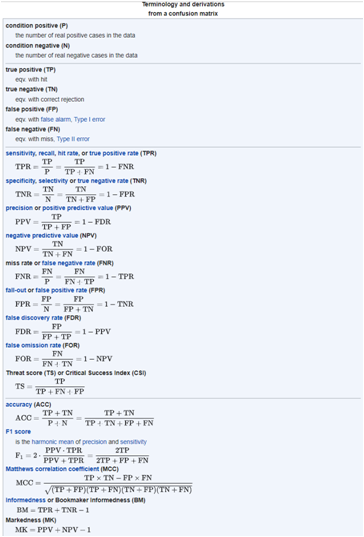
\includegraphics[scale=.55]{Bild31}\\
	                    We’re only scratching the surface here.
	                \end{figure}
	        \end{column}
	        
	    \end{columns}
	\end{frame}
	
	

\end{document}